% Section 6: Systems of Linear Equations $Ax=b$  (original handwritten pages 43--51)
\section{Systems of Linear Equations $Ax=b$}\label{sec:axb}
\syllabusweek{Week 7 --- systems of linear equations of the form $Ax=b$}
\subsection{Existence and Uniqueness of Solutions}\label{ss:exist-unique}
\[
Ax = b, \qquad A\in\C^{m\times n}, \quad x\in\C^n, \quad b\in\C^m
\]
\begin{center}
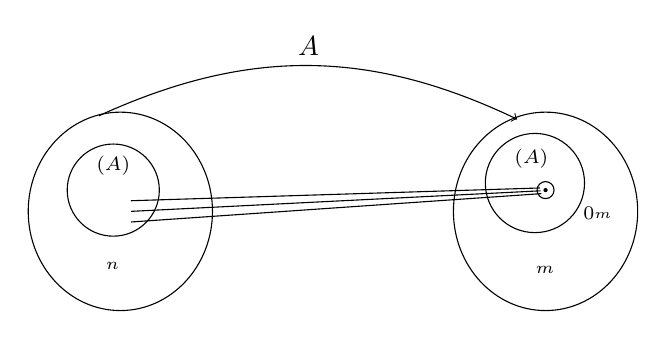
\begin{tikzpicture}[scale=0.9]
  % domain C^n
  \draw (0,0) ellipse (1.3 and 1.4);
  \draw (-0.1,0.3) circle (0.65);
  \node at (-0.1,0.65) {\scriptsize $\Null(A)$};
  \node at (-0.1,-0.85) {\small $\C^n$};
  % codomain C^m
  \draw (6,0) ellipse (1.3 and 1.4);
  \draw (5.85,0.4) circle (0.7);
  \node at (5.8,0.75) {\scriptsize $\Range(A)$};
  \draw (6.0,0.3) circle (0.12);
  \fill (6.0,0.3) circle (0.03);
  \node at (6.75,-0.05) {\scriptsize $0_{\C^m}$};
  % corrected: second small "C^m" label next to the zero vector; read as the subscript of 0 (0_{C^m}), consistent with N(A)={x: Ax=0_{C^m}}
  \node at (6,-0.9) {\small $\C^m$};
  % map
  \draw[->] (-0.3,1.35) to[bend left=25] node[above] {$A$} (5.6,1.3);
  \draw (0.15,0.15) -- (5.92,0.33);
  \draw (0.15,0.0) -- (5.93,0.29);
  \draw (0.15,-0.15) -- (5.94,0.25);
\end{tikzpicture}
\end{center}
\explain{$A$ maps every vector of $\Null(A)$ to $0_{\C^m}$.}
The two fundamental subspaces of $A$:
\begin{align*}
\text{\term{range space}: }\Range(A) &= \{y\in\C^m \mid \exists x\in\C^n \text{ satisfying } y=Ax\}\\
\text{\term{null space}: }\Null(A) &= \{x\in\C^n \mid Ax = 0_{\C^m}\}
\end{align*}
Rank--nullity:
\begin{gather*}
\underbrace{\dim(\Range(A))}_{\text{rank}} + \underbrace{\dim(\Null(A))}_{\text{nullity}} = n = \#\text{ of columns of } A
\end{gather*}
Recall also, for a subspace $M$ of $\V$:
\begin{align*}
&\V = M\overset{\perp}{\oplus}M^\perp\\
&v = v_1+v_2, \qquad v_1\in M, \quad v_2\in M^\perp, \qquad v_1,v_2 \text{ are unique}\\
&v_1\perp v_2, \qquad \dim M + \dim M^\perp = \dim \V
\end{align*}
Two questions:
\begin{enumerate}[label=\arabic*-), nosep]
  \item Is there an exact solution? \ ($\Range(A)$)
  \item If there is, is it unique? \ ($\Null(A)$)
\end{enumerate}
\explain{Question 1 is answered by $\Range(A)\subseteq\C^m$ (the codomain side), question 2 by $\Null(A)\subseteq\C^n$ (the domain side).}

% ===== Page 43 =====
\sep
\point $\displaystyle \underbrace{\bmat{1\\1}}_{A}\underset{\in\R}{x} = \underbrace{\bmat{2\\2}}_{b}$,
\qquad $b\in\Range(A)$\origpage{43}\\[4pt]
$\Rightarrow$ $\exists$ an exact solution. \quad $\Rightarrow$ The solution is unique.

\point $\displaystyle \underbrace{\bmat{1\\1}}_{A}x = \underbrace{\bmat{2\\1}}_{b}$
\quad $\Rightarrow$ No exact solution! \qquad $b\notin\Range(A)$
\begin{align*}
y = Ax &= \big[\,a_1 \,\vdots\, a_2 \,\vdots\, a_3 \,\vdots\, \cdots \,\vdots\, a_n\,\big]\bmat{x_1\\x_2\\ \vdots\\ x_n}
= x_1\vec a_1 + x_2\vec a_2 + \dots + x_n\vec a_n\\[4pt]
\Range(A) &= \Span\{\vec a_1,\vec a_2,\dots,\vec a_n\} \triangleq \text{\term{column space} of } A\\
\Range(A) &= \Span\left\{\bmat{1\\1}\right\}, \qquad \bmat{2\\1}\notin\Range(A)
\end{align*}

\begin{keybox}
$\therefore$ 1-) \key{There exists an exact solution iff $b\in\Range(A)$.}
\end{keybox}

\point $\displaystyle \underbrace{\bmat{1&2\\1&2}}_{A}\underset{\in\R^2}{x} = \underbrace{\bmat{2\\2}}_{b}$:
\quad $\Range(A) = \Span\left\{\bmat{1\\1}\right\}$ \& $b\in\Range(A)$ $\Rightarrow$ $\therefore\ \exists$ an exact solution
\[
x_1 = \bmat{2\\0} \quad\text{or}\quad x_2 = \bmat{0\\1} \quad\text{or}\quad x_3 = \bmat{4\\-1} \quad\dots
\]

\needspace{14\baselineskip}
\sep
Dimensions in the first example:
\begin{gather*}
\left.\begin{aligned}
A &= \bmat{1\\1}, \qquad \dim\C = 1\\
\Range(A) &= \Span\left\{\bmat{1\\1}\right\}, \qquad \dim\Range(A) = 1
\end{aligned}\right\}
\quad
\begin{aligned}
&\underbrace{\dim(\Range(A))}_{1} + \underbrace{\dim(\Null(A))}_{0} = 1 \leftarrow \#\text{ of columns}\\
&\Null(A) = \{0\}, \qquad \dim(\Null(A)) = 0
\end{aligned}
\end{gather*}
and in the third example:
\begin{align*}
&A = \bmat{1&2\\1&2}, \qquad \Range(A) = \Span\left\{\bmat{1\\1}\right\}, \qquad \dim\Range(A) = 1\\
&\underbrace{\dim\Range(A)}_{1} + \underbrace{\dim\Null(A)}_{1} = 2, \qquad
\Null(A) = \Span\left\{\bmat{2\\-1}\right\}\\[4pt]
&x_1-x_2 = \bmat{2\\-1}, \qquad x_1-x_3 = \bmat{-2\\1}, \qquad x_2-x_3 = \bmat{-4\\2} \qquad \text{all inside null space.}
\end{align*}

\needspace{10\baselineskip}
\sep
In general:
\begin{align*}
&A\hat x = b \qquad \hat x \text{ is exact}\\
&\underset{\substack{\uparrow\\ \in\Null(A)}}{\hat x + m} \;\Rightarrow\; A(\hat x+m) = A\hat x + \underbrace{\overset{\in\Null(A)}{Am}}_{0} = b+0 = b
\end{align*}
% corrected: notes had "= b+0 = 0" at the end (meant "= b") and "x is exact" (meant \hat x)
\begin{itemize}[nosep]
  \item if $\hat x$ satisfies $A\hat x = b$ exactly $\Rightarrow$ $\hat x + m$ satisfies $A(\hat x+m) = b$ exactly \ ($m\in\Null(A)$);
  \item if $m\neq 0 \Rightarrow \hat x \neq \hat x + m$;
  \item if $\Null(A)$ includes nonzero vectors $\Rightarrow$ \key{infinitely many exact solutions}.
\end{itemize}

% ===== Page 44 =====
\origpage{44}
\begin{keybox}
$\therefore$ 2-) If an exact solution $\hat x$ exists, then \key{it is unique
$\iff \Null(A) = \{0\}$} \ or \ $\dim\Null(A) = 0$.
\end{keybox}
\needspace{7\baselineskip}
\begin{insight}
Conversely, if $A\hat x = b$ and $A\tilde x = b$, then $A(\hat x-\tilde x) = 0$, i.e.\ any two exact solutions
differ by a vector of $\Null(A)$. Hence \key{the full solution set is the affine set
$\{\hat x + m : m\in\Null(A)\}$}. By rank--nullity, $\Null(A)=\{0\}$ iff $\rank A = n$ (the columns of $A$ are
linearly independent); this requires $m\ge n$.
\end{insight}

\subsection{Least-Squares Solutions}\label{ss:least-squares}
\point $\displaystyle \bmat{1\\1}x = \bmat{2\\1}$, \qquad $Ax = b$, \qquad $b\notin\Range(A)$

\paragraph{\term{Least-squares problem}.}
\[
\min_{x\in\C^n} \underbrace{\norm{Ax-b}^{2}}_{\text{error}}
\]
\explain{The exponent $2$ doesn't matter; $\norm{\cdot}$ is the induced norm of the inner product.}
\[
\hat x = \arg\min_{x\in\C^n}\norm{Ax-b}
\]
\explain{$\hat x$: \term{minimum error solution} / \term{least-squares solution}.}
Since $b\in\C^m$, decompose it:
\begin{align*}
\C^m &= M\overset{\perp}{\oplus}M^\perp\\
\C^m &= \Range(A)\overset{\perp}{\oplus}\Range^\perp(A)\\
b &= \underset{\in\Range(A)}{b_1} + \underset{\in\Range^\perp(A)}{b_2}
\;\Rightarrow\; b_1 = \operatorname{Proj}_{\Range(A)} b, \quad b_2 = \operatorname{Proj}_{\Range^\perp(A)} b
\;\Rightarrow\; b_1\perp b_2
\end{align*}
\needspace{15\baselineskip}
Then
\begin{align*}
\norm{Ax-b}^2 &= \inner{Ax-b}{Ax-b}\\
&= \big\langle (\underset{\in\Range(A)}{Ax}-\underset{\in\Range(A)}{b_1}) - \underset{\in\Range^\perp(A)}{b_2},\ (Ax-b_1)-b_2\big\rangle
&& (\Range(A) \text{ is a subspace})\\
&= \inner{Ax-b_1}{Ax-b_1}\\
&\quad \cancel{-\inner{Ax-b_1}{b_2}}\\
&\quad \cancel{-\inner{b_2}{Ax-b_1}} && (\to 0 \text{ because of orthogonality})\\
&\quad +\inner{b_2}{b_2}\\
&= \inner{Ax-b_1}{Ax-b_1} + \inner{b_2}{b_2}\\
&= \overbrace{\Big\lVert A\underset{\substack{\uparrow\\ \text{find an } x}}{x}-\underset{\in\Range(A)}{b_1}\Big\rVert^2}^{\text{zero}} + \norm{b_2}^2 \geq \norm{b_2}^2
\end{align*}
% corrected: notes had the first term without the square, i.e. ||Ax-b_1|| + ||b_2||^2
\explain{\key{The first term can be made zero}: $b_1\in\Range(A)$, so some $x$ satisfies $Ax=b_1$ exactly.}
\needspace{8\baselineskip}
Therefore
\begin{gather*}
\boxed{\min_{x\in\C^n}\norm{Ax-b} = \norm{b_2} = \norm{\operatorname{Proj}_{\Range^\perp(A)} b}}\\*[4pt]
A\hat x = b_1, \qquad \hat x = \arg\min_{x\in\C^n}\norm{Ax-b}, \qquad
b_1 = \operatorname{Proj}_{\Range(A)} b\\*[4pt]
\underbrace{\hat x}_{\substack{\text{min error /}\\ \text{least-squares solution}}} = \arg\min_{x\in\C^n}\norm{Ax-b}
\end{gather*}
\begin{insight}[Normal equations]
$A\hat x = b_1$ is equivalent to $b - A\hat x = b_2 \perp \Range(A)$, i.e.\ $a_j\Hm(b-A\hat x) = 0$ for every
column $a_j$ of $A$:
\[
A\Hm(b-A\hat x) = 0 \quad\Longleftrightarrow\quad \boxed{A\Hm A\,\hat x = A\Hm b}
\]
(the same equations as $B\Hm B\alpha^* = B\Hm x$ before, with $B=A$). \key{These normal equations always have a
solution.} If the columns of $A$ are linearly independent, $A\Hm A$ is invertible and
$\hat x = (A\Hm A)^{-1}A\Hm b$ is unique; otherwise there are infinitely many least-squares solutions,
differing by elements of $\Null(A\Hm A)=\Null(A)$.
\end{insight}

% ===== Page 45 =====
\sep
\point $\displaystyle \bmat{1\\1}x = \bmat{2\\1}$, \qquad $b\notin\Range(A)$, \qquad
$\Range(A) = \Span\left\{\bmat{1\\1}\right\}$\origpage{45}
\begin{align*}
&P_{\Range(A)} = B(B\Hm B)^{-1}B\Hm, \qquad B = \bmat{1\\1}, \qquad B\Hm B = \bmat{1&1}\bmat{1\\1} = 2\\
&P_{\Range(A)} = \bmat{1\\1}\frac12\bmat{1&1} = \bmat{1/2&1/2\\1/2&1/2}\\
&b_1 = P_{\Range(A)}b = \bmat{1/2&1/2\\1/2&1/2}\bmat{2\\1} = \bmat{3/2\\3/2}\\
&\underbrace{\bmat{1\\1}}_{A}\hat x = \underbrace{\bmat{3/2\\3/2}}_{b_1},
\qquad \hat x = \frac32
\end{align*}
\explain{$\hat x = \tfrac32$ is the average of the entries of $b = \bmat{2 & 1}\T$.}
\explain{Same result from the normal equations: $A\Hm A = 2$, $A\Hm b = 3$ $\Rightarrow$ $\hat x = \tfrac32$; $b-b_1 = \bmat{1/2 & -1/2}\T$, so the minimum error is $\norm{b-b_1} = \tfrac1{\sqrt2}$.}

\point $\displaystyle \bmat{1\\1}x = \bmat{2\\1}$, \qquad
$\Range(A) = \Span\left\{\bmat{1\\1}\right\}$
\[
b_1 = P_{\Range(A)}b = \bmat{1/2&1/2\\1/2&1/2}\bmat{2\\1} = \bmat{3/2\\3/2}
\]
% corrected: notes had the multiplied vector as [1;1] (it is b=[2;1])
Then
\begin{alignat*}{2}
&A\hat x = b_1, &\qquad& \hat x = 3/2\\
&\Null(A) = \{0\},\ \dim\Null(A) = 0 &\qquad& \Rightarrow\ \hat x \text{ \key{is unique.}}
\end{alignat*}

\point $\displaystyle \bmat{1&2\\1&2}x = \bmat{2\\1}$, \qquad
$\Range(A) = \Span\left\{\bmat{1\\1}\right\}$, \qquad $b\notin\Range(A)$
\begin{align*}
&b_1 = P_{\Range(A)}b = \bmat{3/2\\3/2}\\
&\bmat{1&2\\1&2}\hat x = \bmat{3/2\\3/2}
\quad\Rightarrow\quad \hat x = \bmat{3/2\\0}, \quad \hat x = \bmat{0\\3/4}, \quad \hat x = \bmat{1/2\\1/2}\\
&\Null(A) = \Span\left\{\bmat{2\\-1}\right\}
\quad\Rightarrow\quad \hat x \text{ \key{is not unique!}}
\end{align*}
\explain{All least-squares solutions: $\hat x = \bmat{3/2 & 0}\T + t\bmat{2 & -1}\T$, $t\in\R$ (e.g.\ $t=-\tfrac34$ gives $\bmat{0 & 3/4}\T$, $t=-\tfrac12$ gives $\bmat{1/2 & 1/2}\T$). Each leaves the same error $\norm{b_2} = \tfrac1{\sqrt2}$.}

\subsection{Minimum-Norm Solutions}\label{ss:min-norm}
\paragraph{\term{Minimum-norm solution}.}
\begin{gather*}
b\in\Range(A) \;\Rightarrow\; \min_{Ax=b}\norm{x}, \qquad
\hat x_1 = \arg\min_{Ax=b}\norm{x}, \qquad x = \hat x + \overset{\in\Null(A)}{m}\\[4pt]
\min_{m\in\Null(A)}\norm{\hat x + m}, \qquad A\hat x = b
\end{gather*}
\explain{When there are infinitely many solutions, pick the one with the smallest norm. Every solution has the form $\hat x+m$ for one fixed solution $\hat x$, so we minimize over $m\in\Null(A)$.}
\begin{center}
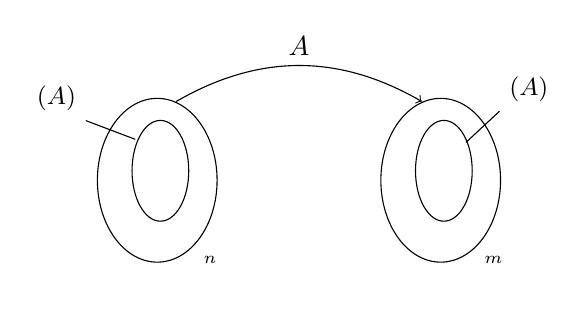
\begin{tikzpicture}[scale=0.8]
  \draw (0,0) ellipse (0.95 and 1.3);
  \draw (0.05,0.15) ellipse (0.45 and 0.8);
  \node at (0.85,-1.35) {\small $\C^n$};
  \node (NA) at (-1.6,1.3) {\small $\Null(A)$};
  \draw (-0.35,0.65) -- (NA.south east);
  \draw (4.5,0) ellipse (0.95 and 1.3);
  \draw (4.55,0.15) ellipse (0.45 and 0.8);
  \node at (5.35,-1.35) {\small $\C^m$};
  \node (RA) at (5.9,1.45) {\small $\Range(A)$};
  \draw (4.9,0.6) -- (RA.south west);
  \draw[->] (0.3,1.25) to[bend left=30] node[above] {$A$} (4.2,1.25);
\end{tikzpicture}
\end{center}
\begin{align*}
&\C^m = \Range(A)\overset{\perp}{\oplus}\Range^\perp(A)\\
&\C^n = \Null^\perp(A)\overset{\perp}{\oplus}\Null(A)\\
&\hat x = \underset{\in\Null^\perp(A)}{\hat x_1} + \underset{\in\Null(A)}{\hat x_2},
\qquad \hat x_1 = \operatorname{Proj}_{\Null^\perp(A)}\hat x, \quad \hat x_2 = \operatorname{Proj}_{\Null(A)}\hat x,
\qquad \hat x_1\perp\hat x_2
\end{align*}

% ===== Page 46 =====
Then\origpage{46}
\begin{align*}
\norm{\hat x + m}^2 &= \inner{\hat x + m}{\hat x + m}\\
&= \big\langle \underset{\in\Null^\perp}{\hat x_1} + (\underset{\in\Null}{\hat x_2} + \underset{\in\Null}{m}),\ \underset{\in\Null^\perp}{\hat x_1} + (\underset{\in\Null}{\hat x_2} + \underset{\in\Null}{m})\big\rangle\\
&= \inner{\hat x_1}{\hat x_1} + \inner{\hat x_2 + m}{\hat x_2 + m}\\
&= \norm{\hat x_1}^2 + \norm{\hat x_2 + m}^2\\
&\geq \norm{\hat x_1}^2
\end{align*}
\explain{Equality for $m^* = -\hat x_2 \;\Rightarrow\; \norm{\hat x_2 + m} = 0$.}
Hence
\begin{gather*}
\min_{\substack{Ax=b\\ m\in\Null(A)}} \norm{\hat x + m} = \norm{\hat x - \hat x_2} = \norm{\hat x_1}
\end{gather*}
and $\hat x_1$ is itself a solution:
\begin{align*}
A\hat x &= b\\
A(\hat x_1 + \hat x_2) &= b\\
A\hat x_1 + \underbrace{\cancel{A\hat x_2}}_{0} &= b\\
\Rightarrow\quad A\hat x_1 &= b\\[4pt]
&\boxed{\hat x_1 = \operatorname{Proj}_{\Null^\perp(A)}\hat x = \text{minimum-norm solution}}
\end{align*}
\begin{insight}[Summary of the method]
\begin{itemize}[nosep]
  \item $\hat x_1$ does not depend on which solution $\hat x$ we start from: two solutions differ by an element
        of $\Null(A)$, which the projection onto $\Null^\perp(A)$ removes. So \key{the minimum-norm solution is unique}.
  \item $\Null^\perp(A) = \Range(A\Hm)$ (since $Ax=0 \iff x\perp$ every row of $A$, i.e.\ every column of $A\Hm$).
        Hence the minimum-norm solution can be written $\hat x_1 = A\Hm z$, and $AA\Hm z = b$; if $A$ has
        linearly independent rows, $\hat x_1 = A\Hm(AA\Hm)^{-1}b$.
  \item If $b\notin\Range(A)$, combine both steps: replace $b$ by $b_1 = \operatorname{Proj}_{\Range(A)}b$, take any
        least-squares solution and project it onto $\Null^\perp(A)$. The result is the \term{minimum-norm
        least-squares solution} (this is what the pseudo-inverse $A^{+}b$ computes); the example below does exactly this.
\end{itemize}
\end{insight}

\begin{example}
\begin{gather*}
\bmat{1&2\\1&2}x = \bmat{2\\1}, \qquad
b_1 = \operatorname{Proj}_{\Range(A)} b = \bmat{3/2\\3/2}\\[4pt]
\bmat{1&2\\1&2}\hat x = \bmat{3/2\\3/2}
\quad\Rightarrow\quad
\hat x = \bmat{3/2\\0}\\[4pt]
\Null(A) = \Span\left\{\bmat{2\\-1}\right\}, \qquad
\underbrace{\dim\Null(A)}_{1} + \underbrace{\dim\Null^\perp(A)}_{1} = 2\\[4pt]
\Null^\perp(A) = \Span\Big\{\underbrace{\bmat{1\\2}}_{v}\Big\} = \Range(A\Hm)\\[4pt]
P_{\Null^\perp(A)} = B(B\Hm B)^{-1}B\Hm \;\overset{B=v}{=}\; \frac{vv\Hm}{v\Hm v}
= \frac{\bmat{1\\2}\bmat{1&2}}{\bmat{1&2}\bmat{1\\2}} = \frac15\bmat{1&2\\2&4}\\[4pt]
\hat x_1 = \frac15\bmat{1&2\\2&4}\bmat{3/2\\0} = \frac15\bmat{3/2\\3} = \bmat{3/10\\3/5}
\end{gather*}
\begin{insight}[Checking the answer]
\begin{itemize}[nosep]
  \item $A\hat x_1 = \bmat{3/10+6/5\\ 3/10+6/5} = \bmat{3/2\\3/2} = b_1$, so $\hat x_1$ is a least-squares solution.
  \item $\hat x_1 = \tfrac{3}{10}\bmat{1 & 2}\T\in\Null^\perp(A)$, i.e.\ $\hat x_1\perp\bmat{2 & -1}\T$.
  \item Starting from $\bmat{0 & 3/4}\T$ or $\bmat{1/2 & 1/2}\T$ instead gives the same $\hat x_1$, e.g.
        \[
        \tfrac15\bmat{1&2\\2&4}\bmat{0\\3/4} = \bmat{3/10\\3/5}.
        \]
  \item Norms: $\norm{\hat x_1}^2 = \tfrac{9}{20} = 0.45$, smaller than
        $\norm{\bmat{3/2 & 0}\T}^2 = 2.25$, $\norm{\bmat{0 & 3/4}\T}^2 = 0.5625$ and $\norm{\bmat{1/2 & 1/2}\T}^2 = 0.5$.
\end{itemize}
\end{insight}
\end{example}

% ===== Page 47 =====
\subsection{General Procedure and the Fundamental Theorem}\label{ss:procedure}
\begin{itemize}[leftmargin=1.5em,topsep=0pt]
\item If $b\in\Range(A)$:\origpage{47} \key{$\exists$ an exact solution} to $A\hat{x}=b$.
\item If $b\notin\Range(A)$:
\[
b_1=\operatorname{Proj}_{\Range(A)} b, \qquad A\hat{x}=b_1
\]
\begin{itemize}
\item If $\Null(A)=\{0\}$ $\Rightarrow$ \key{$\hat{x}$ is unique}.
\item If $\Null(A)\neq\{0\}$ $\Rightarrow$ $\hat{x}_1=\operatorname{Proj}_{\Null^\perp(A)}\hat{x}$.
\end{itemize}
\end{itemize}

\begin{center}
\begin{tabular}{@{}l@{\quad}l@{}}
$\hat{x}$: & \term{minimum error solution} (least-squares)\\
$\hat{x}_1$: & \term{minimum error-norm solution}
\end{tabular}
\end{center}

\begin{insight}[Why the procedure works]
\begin{itemize}[nosep,leftmargin=1.2em]
\item The error $b-A\hat x$ is smallest when $A\hat x$ is the point of $\Range(A)$ closest to $b$, i.e.\ $A\hat x=b_1=\operatorname{Proj}_{\Range(A)}b$ (orthogonality principle: $b-b_1\perp\Range(A)$). Writing this as $A\Hm(b-A\hat x)=0$ gives the \term{normal equations} $A\Hm A\hat x=A\Hm b$.
\item If $\Null(A)\neq\{0\}$, every $\hat x+n$ with $n\in\Null(A)$ gives the same $A\hat x=b_1$, so the least-squares solution is not unique. Splitting $\hat x=\hat x_1+\hat x_2$ with $\hat x_1\in\Null^\perp(A)$, $\hat x_2\in\Null(A)$ gives $A\hat x_1=A\hat x=b_1$ and, by Pythagoras, $\norm{\hat x+n}^2=\norm{\hat x_1}^2+\norm{\hat x_2+n}^2\geq\norm{\hat x_1}^2$. Hence \key{$\hat x_1$ is the least-squares solution of minimum-norm}, and it does not depend on which $\hat x$ we started from.
\end{itemize}
\end{insight}

\begin{example}
$A=\bmat{1&2&3\\1&2&3}$, \qquad $n=3$, $m=2$ \quad ($A\in\C^{m\times n}$: $n$ columns, $m$ rows).
\begin{align*}
\Range(A)&=\Span\left\{\bmat{1\\1}\right\}, \qquad \dim(\Range(A))=1\\
\Null(A)&=\Span\left\{\bmat{3\\0\\-1},\bmat{2\\-1\\0}\right\}
\end{align*}
\[
\underbrace{\dim(\Range(A))}_{1}+\underbrace{\dim(\Null(A))}_{2}=3,
\qquad
\underbrace{\dim(\Null(A))}_{2}+\underbrace{\dim(\Null^\perp(A))}_{1}=3
\]
For $\Null^\perp(A)$, a vector $[a\ b\ c]\T$ orthogonal to both basis vectors of $\Null(A)$:
\[
\begin{aligned}3a-c&=0\\2a-b&=0\end{aligned}
\quad\Rightarrow\quad
\begin{aligned}c&=3a\\b&=2a\end{aligned}
\quad\Rightarrow\quad \bmat{a\\b\\c}=a\underbrace{\bmat{1\\2\\3}}_{\text{row of }A}
\qquad\Rightarrow\qquad
\Null^\perp(A)=\Span\left\{\bmat{1\\2\\3}\right\}
\]
\[
\Null^\perp(A)=\Range(A\Hm)
\]
\explain{$\therefore$ \key{Fundamental theorem of linear algebra.}}
\[
\hat{x}_1=\operatorname{Proj}_{\Null^\perp(A)}\hat{x}
=\operatorname{Proj}_{\Range(A\Hm)}\hat{x}
\]
\explain{$\Range(A\Hm)$: row space of $A$.}
\end{example}

\paragraph{Dimensions and rank.} For $A\in\C^{m\times n}$:
\begin{align*}
\dim(\underbrace{\Range(A)}_{k})+\dim(\underbrace{\Null(A)}_{n-k}) &= \#\text{ of columns}=n\\
\dim(\underbrace{\Null(A)}_{n-k})+\dim(\underbrace{\Range(A\Hm)}_{k})&=n
\qquad \big(\dim(\Null(A))+\dim(\Null^\perp(A))=n\big)
\end{align*}
\[
\left.\begin{aligned}
\dim(\Range(A))&=\#\text{ of lin.\ indep.\ columns of }A=\text{column rank}=k\\
\dim(\Range(A\Hm))&=\#\text{ of lin.\ indep.\ rows of }A=\text{row rank}=k
\end{aligned}\right\}\ k=\text{\term{rank} of a matrix}
\]
\[
\#\text{ linearly indep.\ rows}=\#\text{ linearly indep.\ columns}
\quad\text{as}\quad \dim\Range(A)=k=\dim\Range(A\Hm)
\]
$k$: \key{\# of linearly independent rows $=$ \# of linearly independent columns} (column rank $=$ row rank).

% ===== Page 48 =====
\begin{theorem}[Fundamental theorem of linear algebra]\leavevmode\origpage{48}
$\Range(A\Hm)=\Null^\perp(A)$
\end{theorem}
\begin{proof}
$\inner{x}{y}\triangleq y\Hm x$.
\[
\inner{\underset{\C^m}{Ax}}{\underset{\C^m}{y}}_{\C^m}=y\Hm Ax=(A\Hm y)\Hm x=\inner{\underset{\C^n}{x}}{\underset{\C^n}{A\Hm y}}_{\C^n}
\]
Prove $\Null(A)=\Range^\perp(A\Hm)$, which is easier to prove.
\[
\left.\begin{aligned}
\Null(A)&\subset\Range^\perp(A\Hm)\\
\Range^\perp(A\Hm)&\subset\Null(A)
\end{aligned}\right\}\ \text{prove both}\ \Rightarrow\ \Null(A)=\Range^\perp(A\Hm)
\]

\paragraph{Part 1.} $x\in\Null(A)\Rightarrow Ax=0$.

\begin{minipage}{0.25\textwidth}
\centering
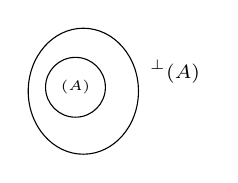
\begin{tikzpicture}
\draw (0,0) ellipse (0.7 and 0.8);
\draw (-0.1,0.05) circle (0.38);
\node[font=\tiny] at (-0.1,0.05) {$\Null(A)$};
\node[font=\scriptsize,anchor=west] at (0.72,0.25) {$\Range^\perp(A\Hm)$};
\end{tikzpicture}
\end{minipage}\hfill
\begin{minipage}{0.72\textwidth}
\begin{align*}
&\inner{Ax}{y}\quad\text{where }\forall y\in\C^m\\
&\inner{Ax}{y}=0\\
&\inner{x}{A\Hm y}=0\quad\forall y\in\C^m\\
\Rightarrow\ & x\perp A\Hm y\quad\forall y\in\C^m\\
\Rightarrow\ & x\perp\Range(A\Hm)\Rightarrow x\in\Range^\perp(A\Hm)
\end{align*}
\end{minipage}

\paragraph{Part 2.} $x\in\Range^\perp(A\Hm)$.

\begin{minipage}{0.25\textwidth}
\centering
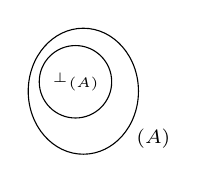
\begin{tikzpicture}
\draw (0,0) ellipse (0.7 and 0.8);
\draw (-0.1,0.12) circle (0.46);
\node[font=\tiny] at (-0.1,0.12) {$\Range^\perp(A\Hm)$};
\node[font=\scriptsize,anchor=west] at (0.55,-0.6) {$\Null(A)$};
\end{tikzpicture}
\end{minipage}\hfill
\begin{minipage}{0.72\textwidth}
\begin{align*}
&x\in\Range^\perp(A\Hm)\\
\Rightarrow\ & x\perp A\Hm y\quad\forall y\in\C^m\\
&\inner{x}{A\Hm y}=0\quad\forall y\in\C^m\\
&\inner{Ax}{y}=0\quad\forall y\in\C^m
\end{align*}
\explain{$Ax\in\C^m$, so choose $y=Ax$:}
\[
\inner{Ax}{Ax}=\norm{Ax}^2=0\Rightarrow Ax=0\Rightarrow x\in\Null(A)
\]
\end{minipage}

Both inclusions hold, so $\Null(A)=\Range^\perp(A\Hm)$. Taking orthogonal complements of both sides (in finite dimensions $(S^\perp)^\perp=S$ for a subspace $S$) gives $\Null^\perp(A)=\Range(A\Hm)$.
\end{proof}

\begin{center}
\begin{minipage}{0.46\textwidth}
\centering
\begin{tikzpicture}[scale=0.85]
\draw (0,0) ellipse (1.1 and 1.25);
\draw (0.05,0.15) ellipse (0.6 and 0.8);
\node[font=\scriptsize] at (0.05,-0.85) {$\Null(A)$};
\node at (0.9,-1.45) {$\C^n$};
\draw (3.8,0) ellipse (1.0 and 1.25);
\draw (3.75,0.15) ellipse (0.6 and 0.8);
\node[font=\scriptsize] at (3.75,-0.85) {$\Range(A)$};
\node at (4.75,-1.45) {$\C^m$};
\fill (3.55,0.45) circle (1.2pt) node[right,font=\scriptsize]{$0$};
\draw[-{Stealth[length=1.5mm]}] (-0.3,0.55) to[bend left=6] (3.5,0.47);
\draw[-{Stealth[length=1.5mm]}] (-0.25,0.25) to[bend left=3] (3.5,0.45);
\draw[-{Stealth[length=1.5mm]}] (-0.2,0.0) to[bend right=4] (3.5,0.43);
\draw[-{Stealth[length=2mm]}] (0.3,1.5) to[bend left=15] node[above]{$A$} (3.4,1.45);
\end{tikzpicture}
\end{minipage}\hfill
\begin{minipage}{0.5\textwidth}
\begin{align*}
&\dim(\overset{k}{\Range(A)})+\dim(\overset{n-k}{\Null(A)})=n\\
&\dim(\Null(A))+\dim(\Null^\perp(A))=n\\
&\underbrace{\dim(\Range(A\Hm))}_{k}+\underbrace{\dim(\Null(A))}_{n-k}=n\\
&\underbrace{\dim(\Range(A))}_{\text{column rank}}=\underbrace{\dim(\Range(A\Hm))}_{\text{row rank}}=k
\end{align*}
\explain{$k$: rank.}
\end{minipage}
\end{center}

\subsection{Special Cases by Rank}\label{ss:rank-cases}
\subsubsection{Case I: Full Column Rank}
$A$ is/has \term{full column rank}: columns of $A$ are linearly independent.
\[
m\Big\{\underbrace{\overset{n}{\bmat{\ &\ &\ \\ \ &\ &\ \\ \ &\ &\ }}}_{\text{tall matrix}}
\overset{n}{\bmat{\ \\ \ \\ \ }}=\bmat{\ \\ \ \\ \ }\Big\}m \qquad m\geq n
\]
\begin{itemize}[nosep,leftmargin=1.5em]
\item $n=\#$ of unknowns, \quad $m=\#$ of equations
\item $m>n$: \term{overdetermined} system of equations
\end{itemize}
Assume
\[
\bmat{a&b&c\\d&e&f}\qquad\text{3 vectors cannot be linearly indep.\ for }\R^2.
\]
\explain{Under the columns: ``2 dim'', ``2 dimension''. Each column lies in $\R^2$, so at most $2$ of them can be linearly independent; full column rank therefore forces $m\geq n$.}

% ===== Page 49 =====
\origpage{49}
\begin{align*}
&\dim(\Range(A))=n\\
&\dim(\Null(A))=0\Rightarrow \Null(A)=\{0\} \qquad A\text{ is one-to-one}
\end{align*}
\key{If we have an exact solution, then the solution is unique.}

If $b\notin\Range(A)$:
\begin{align*}
P_{\Range(A)}&=B(B\Hm B)^{-1}B\Hm\\
\intertext{with $B=A$:}
P_{\Range(A)}&=A(A\Hm A)^{-1}A\Hm\\
b_1=P_{\Range(A)}b&=A(A\Hm A)^{-1}A\Hm b \qquad (A\hat{x}=b_1)\\
\Rightarrow\quad A\big(\underbrace{\hat{x}-(A\Hm A)^{-1}A\Hm b}_{\in\Null(A)}\big)&=0\\
\Rightarrow\quad \hat{x}-(A\Hm A)^{-1}A\Hm b&=0
\ \Rightarrow\ \boxed{\hat{x}=(A\Hm A)^{-1}A\Hm b}
\end{align*}
\explain{Unique solution as $\Null(A)=\{0\}$.}
$(A\Hm A)^{-1}A\Hm$: \term{left pseudo inverse} of $A$.

\begin{insight}
\begin{itemize}[nosep,leftmargin=1.2em]
\item \key{$A\Hm A$ ($n\times n$) is invertible exactly when $A$ has full column rank}: $A\Hm Ax=0\Rightarrow x\Hm A\Hm Ax=\norm{Ax}^2=0\Rightarrow Ax=0\Rightarrow x=0$.
\item The same formula comes directly from the normal equations $A\Hm A\hat x=A\Hm b$.
\item ``Left'' inverse: $\big((A\Hm A)^{-1}A\Hm\big)A=I_n$. If $b\in\Range(A)$, it returns the exact solution.
\end{itemize}
\end{insight}

\subsubsection{Case II: Full Row Rank}
$A$ is/has \term{full row rank}: all rows of $A$ are linearly independent.
\[
m\Big\{\underbrace{\overset{n}{\bmat{\ &\ &\ &\ \\ \ &\ &\ &\ }}}_{\text{fat matrix}}
\bmat{\ \\ \ \\ \ \\ \ }=\bmat{\ \\ \ } \qquad m\leq n
\]
\begin{itemize}[nosep,leftmargin=1.5em]
\item $m$: \# of equations, \quad $n$: \# of unknowns
\item $m<n$: \term{underdetermined} system of equations
\end{itemize}
\begin{align*}
\dim(\Range(A\Hm))&=m\\
\dim(\Range(A))&=m \ \Rightarrow\ \Range(A)=\C^m
\end{align*}
\[
b\in\Range(A)\quad\forall b\in\C^m\Rightarrow\text{\key{Always has an exact solution} (at least one): $A$ is onto.}
% corrected: notes had "b in C^m  for all b in R(A)" (quantifiers swapped)
\]
\begin{align*}
\hat{x}_1&=\operatorname{Proj}_{\Null^\perp(A)}\hat{x}=\operatorname{Proj}_{\Range(A\Hm)}\hat{x}\\
% corrected: notes had Proj_{R(A^H)} x-hat = Proj_{R(A^H)} x-hat (first projection meant onto N^perp(A))
\intertext{with $B=A\Hm$:}
P_{\Range(A\Hm)}&=A\Hm(AA\Hm)^{-1}A\\
\hat{x}_1&=A\Hm(AA\Hm)^{-1}\underbrace{A\hat{x}}_{b}\ \Rightarrow\ \hat{x}_1=A\Hm(AA\Hm)^{-1}b
\end{align*}
$A\Hm(AA\Hm)^{-1}$: \term{right pseudo inverse} of $A$.

\begin{insight}
\begin{itemize}[nosep,leftmargin=1.2em]
\item $AA\Hm$ ($m\times m$) is invertible since the rows of $A$ are independent (same argument as for $A\Hm A$, applied to $A\Hm$).
\item ``Right'' inverse: $A\big(A\Hm(AA\Hm)^{-1}\big)=I_m$, so $A\hat x_1=b$ is indeed an exact solution.
\item $\hat x_1=A\Hm\big((AA\Hm)^{-1}b\big)\in\Range(A\Hm)=\Null^\perp(A)$, so \key{it is the minimum-norm one} among the infinitely many exact solutions $\hat x_1+\Null(A)$.
\end{itemize}
\end{insight}

\subsubsection{Case III: Full Column and Full Row Rank}
$A$ is/has both full column and row rank.
\[
\left.\begin{aligned}m&\geq n\\ n&\geq m\end{aligned}\right\}\ m=n:\quad
\begin{aligned}
&A\text{ is a square matrix}\\
&\left.\begin{aligned}&A\text{ is one-to-one}\\&A\text{ is onto}\end{aligned}\right\}
\ \begin{aligned}&A\text{ has an inverse}\\&A\text{ is invertible.}\end{aligned}
\end{aligned}
\]
\explain{Both pseudo inverses reduce to $A^{-1}$ here: $(A\Hm A)^{-1}A\Hm=A^{-1}(A\Hm)^{-1}A\Hm=A^{-1}$ and $A\Hm(AA\Hm)^{-1}=A^{-1}$.}
\key{Exact solution exists. The solution is unique.}
\[
Ax=b,\qquad x_1=\hat{x}=x=A^{-1}b
\]

% ===== Page 50 =====
\begin{example}\leavevmode\origpage{50}
\[
\underset{A}{\bmat{1&2\\1&2}}\underset{x}{\bmat{x_1\\x_2}}=\underset{b}{\bmat{1\\1}},
\qquad
\Range(A)=\Span\left\{\bmat{1\\1}\right\},\quad b\in\Range(A)
\ \Rightarrow\ \text{has exact solution},\quad \hat{x}=\bmat{1\\0}
\]
\begin{minipage}[c]{0.50\textwidth}
\raggedright
$\begin{aligned}
&\dim\Range(A)=1\\
&\dim\Null(A)=1\\
&\Null(A)=\Span\left\{\bmat{-2\\1}\right\}\\
&\hat{x}+n=\bmat{1\\0}+\alpha\bmat{-2\\1},\quad n\in\Null(A)
% corrected: notes had "x-hat + m" (an element of N(A) is added)
\end{aligned}$
\explain{In the sketch: $\Range(A\Hm)=\Span\{[1\ 2]\T\}$; the solution set $\hat x+\Null(A)$ is the line through $\hat x=[1\ 0]\T$ parallel to $\Null(A)$; $\hat{x}_1=\tfrac15[1\ 2]\T$ is its point on $\Range(A\Hm)$, and $\hat{x}_2=\hat x-\hat x_1\in\Null(A)$ is the part to ``get rid of''.}
\end{minipage}\hfill
\begin{minipage}[c]{0.48\textwidth}
\centering
\begin{tikzpicture}[scale=0.9,>={Stealth[length=1.6mm]}]
\draw[->] (-2.5,0)--(2.7,0) node[right]{$x_1$};
\draw[->] (0,-1.7)--(0,2.2) node[above]{$x_2$};
% R(A^H): y = 2x
\draw[very thick,blue!50!black] (-0.85,-1.7)--(1.05,2.1) node[above right,font=\scriptsize]{$\Range(A\Hm)$};
% N(A): y = -x/2 through origin
\draw (-2.5,1.25)--(2.7,-1.35) node[below,font=\scriptsize]{$\Null(A)$};
% solution set: through (1,0), slope -1/2
\draw[gray!70!black] (-1.8,1.4)--(2.7,-0.85) node[right,font=\scriptsize]{$\hat x+\Null(A)$};
% ticks
\foreach \t in {-2,1,2} \draw (\t,0.06)--(\t,-0.06);
\node[font=\tiny,below] at (-2,0) {$-2$};
\node[font=\tiny,above] at (2,0) {$2$};
\node[font=\tiny,above right] at (1,0) {$1$};
\draw[dashed,gray] (-2,0)--(-2,1)--(0,1);
\draw[dashed,gray] (2,0)--(2,-1)--(0,-1);
% right angle at x1hat
\draw ($(0.2,0.4)+(-0.0894,-0.1789)$) -- ++(0.1789,-0.0894) -- ++(0.0894,0.1789);
\fill (0.2,0.4) circle (1.4pt);
\node[font=\scriptsize,left] at (0.05,0.55) {$\hat{x}_1$};
\fill (1,0) circle (1.4pt);
\node[font=\scriptsize,below] at (1.1,0) {$\hat{x}$};
\draw[->,dashed,thick] (0,0)--(0.8,-0.4) node[font=\scriptsize,below]{$\hat{x}_2$};
\end{tikzpicture}
\end{minipage}

\explain{Check: $\hat x_1=\tfrac15[1\ 2]\T$ gives $A\hat x_1=[1\ 1]\T=b$, and $\norm{\hat x_1}^2=\tfrac15<1=\norm{\hat x}^2$; the right pseudo inverse cannot be used here since $AA\Hm=\left[\begin{smallmatrix}5&5\\5&5\end{smallmatrix}\right]$ is singular ($A$ has rank 1, neither full row nor full column rank), so the projection route is used.}
\end{example}

\subsubsection{Case IV: Neither Full Column nor Full Row Rank}
$A$ is/has neither full column rank nor full row rank.

\begin{example}
\[
\underset{A}{\bmat{1&0&1\\1&1&2\\0&1&1}}\underset{x}{\bmat{x_1\\x_2\\x_3}}=\underset{b}{\bmat{1\\0\\3}}
\qquad
\begin{aligned}
&2\text{ linearly indep.\ columns}\\
&2\text{ linearly indep.\ rows}\\
&\dim(\Range(A))=\dim(\Range(A\Hm))=2\\
&\dim(\Null(A))=1\\
&\dim(\Null^\perp(A))=2
\end{aligned}
\]
\[
\bmat{1\\0\\3}=\underset{\alpha}{\underset{\parallel}{1}}\bmat{1\\1\\0}+\underset{\beta}{\underset{\parallel}{3}}\bmat{0\\1\\1}\quad\times
\qquad\Rightarrow\qquad b\notin\Range(A)\Rightarrow\text{\key{No exact solution.}}
\]
\explain{Column 3 $=$ column 1 $+$ column 2, so $\Range(A)=\Span\{[1\ 1\ 0]\T,[0\ 1\ 1]\T\}$. Matching the 1st and 3rd entries of $b$ forces $\alpha=1$, $\beta=3$, but then the 2nd entry would be $\alpha+\beta=4\neq0$.}

\paragraph{Method I.}
\begin{align*}
P_{\Range(A)}&=B(B\Hm B)^{-1}B\Hm\\
B&=\bmat{1&0\\1&1\\0&1},\qquad B\Hm B=\bmat{1&1&0\\0&1&1}\bmat{1&0\\1&1\\0&1}=\bmat{2&1\\1&2}\\
(B\Hm B)^{-1}&=\frac13\bmat{2&-1\\-1&2}\\
P_{\Range(A)}&=\bmat{1&0\\1&1\\0&1}\frac13\bmat{2&-1\\-1&2}\bmat{1&1&0\\0&1&1}=\frac13\bmat{2&1&-1\\1&2&1\\-1&1&2}\\
b_1=P_{\Range(A)}b&=\frac13\bmat{-1\\4\\5}
\end{align*}
\[
\underbrace{\bmat{1&0&1\\1&1&2\\0&1&1}}_{A}\underbrace{\bmat{x_1\\x_2\\x_3}}_{\hat{x}}=\underbrace{\frac13\bmat{-1\\4\\5}}_{b_1}
\qquad\Rightarrow\qquad \underset{\text{minimum error solution.}}{\hat{x}=\frac13\bmat{-1\\5\\0}}
\]
\explain{This was method I. With $x_3=0$: $x_1=-\tfrac13$, $x_1+x_2=\tfrac43\Rightarrow x_2=\tfrac53$, and the 3rd row $x_2+x_3=\tfrac53$ checks. The error is $b-b_1=\tfrac43[1\ {-1}\ 1]\T$, which is orthogonal to both columns of $B$, as it must be.}

\paragraph{Method II.}
\[
\underbrace{\bmat{1&0\\1&1\\0&1}}_{A_1}\underbrace{\bmat{x_1\\x_2}}_{z}=\bmat{1\\0\\3}
\qquad
\begin{aligned}
&\Rightarrow\Null(A_1)=\{0\}\\
&\Rightarrow\text{full column rank}\\
&\Rightarrow\text{Exact solution is known}
\end{aligned}
\]
% corrected: notes had z = [x2; x3]; A_1 consists of the first two columns of A, so z = [x1; x2] (consistent with the final x-hat).
\explain{Idea: drop the dependent third column (set $x_3=0$); the remaining $A_1$ has full column rank and $\Range(A_1)=\Range(A)$, so Case I applies.}
\[
\hat{z}=(A_1\Hm A_1)^{-1}A_1\Hm b=\frac13\bmat{2&-1\\-1&2}\bmat{1&1&0\\0&1&1}\bmat{1\\0\\3}=\underbrace{\frac13\bmat{-1\\5}}_{\hat{z}\ \to\ \text{unique}}
\qquad\therefore\ \hat{x}=\frac13\bmat{-1\\5\\0}
\]

% ===== Page 51 =====
\paragraph{Minimum-norm solution.} $A\Hm=A\T$\origpage{51} as matrix is real.
\begin{align*}
A\Hm&=\bmat{1&1&0\\0&1&1\\1&2&1}\\
P_{\Range(A\Hm)}&=B(B\Hm B)^{-1}B\Hm,\qquad B=\bmat{1&0\\0&1\\1&1}\\
(B\Hm B)^{-1}&=\frac13\bmat{2&-1\\-1&2}\\
P_{\Range(A\Hm)}&=\frac13\bmat{2&-1&1\\-1&2&1\\1&1&2}\\
\hat{x}_1=P_{\Range(A\Hm)}\hat{x}&=\frac19\bmat{-7\\11\\4}
\end{align*}
\explain{$\therefore$ \key{$\hat{x}_1$: minimum error, minimum-norm solution.}}
\begin{insight}[Check]
$A\hat x_1=\tfrac19[-3\ \ 12\ \ 15]\T=\tfrac13[-1\ \ 4\ \ 5]\T=b_1$, so $\hat x_1$ has the same (minimum) error as $\hat x$. Moreover $\hat x-\hat x_1=\tfrac49[1\ \ 1\ {-1}]\T$ spans $\Null(A)$ (indeed $A[1\ 1\ {-1}]\T=0$), and
$\norm{\hat x_1}^2=\tfrac{186}{81}\approx2.30<\tfrac{26}{9}\approx2.89=\norm{\hat x}^2$.
\end{insight}
\end{example}
